\documentclass[addpoints,10pt]{exam}

\usepackage{amsmath,amsthm,enumitem,wrapfig,amsfonts,mathtools}
\usepackage[mathscr]{euscript}
\usepackage[super]{nth}
\usepackage{dsfont}
\usepackage{xparse}
\usepackage{cancel}

\usepackage{geometry}
\usepackage[T1]{fontenc} % Use 8-bit encoding that has 256 glyphs
\renewcommand{\rmdefault}{ptm} %Change the Front Family from the default(cmr) to ptm(Times)
\usepackage{amsmath,amsfonts,amsthm,amssymb} % Math packages
\usepackage{bm}
%\usepackage{mathptmx}
\usepackage{graphicx}
\usepackage{sectsty} % Allows customizing section commands
% \allsectionsfont{\centering} % Make all sections centered, the default font and small caps

\usepackage{pgfplots}
\pgfplotsset{compat=1.18}
\usetikzlibrary{arrows.meta}
\usepackage{xcolor}
\definecolor{darkpastelgreen}{rgb}{0.01, 0.75, 0.24}
\definecolor{blue-violet}{rgb}{0.54, 0.17, 0.89}
%\usepackage{polylongdiv} %polynomial long division
% Custom problem environmenturther
\usepackage{polynom}
\newcounter{cprob}
\newenvironment{cprob}[1]{%
    \setcounter{cprob}{#1}%
    \noindent\textbf{Problem \thecprob.}%
}{%
    \par\bigskip%
}

\theoremstyle{plain}
\newcommand{\theoremname}{Theorem}
\newtheorem{thm}{\protect\theoremname}
  \theoremstyle{definition}
  \newtheorem{prob}[thm]{Problem}
  \newtheorem*{problem*}{Open Problem}
  \theoremstyle{plain}
  \newtheorem{conjecture}[thm]{Conjecture}
  \theoremstyle{plain}
  \newtheorem{lem}[thm]{Lemma}
  \newtheorem*{lem*}{Lemma}
  \newtheorem{obs}[thm]{Observation}
  \newtheorem{cor}[thm]{Corollary}
  \theoremstyle{definition}
\newtheorem{definition}[thm]{Definition}
\newcommand{\subsetdot}{\mathrel{\subset\mkern-13mu\cdot\mkern4mu}}




% Patch prob environment to be single spaced
\let\oldprob\prob
\let\endoldprob\endprob
\renewenvironment{prob}
  {\begin{singlespace}\oldprob}
  {\endoldprob\end{singlespace}}

% start problem one line below like for enumerated problems with multiple parts
\newcommand{\belowtitle}{\leavevmode\newline}
%\Observe command
\newcommand{\Observe}{\text{Observe.}}
%(=>)
\newcommand{\IF}{\mathbf{(\Rightarrow)}}
%(<=)
\newcommand{\FI}{\mathbf{(\Leftarrow)}}
%equivalence classes; \class[S]{ *content in square brackets* }
\newcommand{\class}[2][]{\ensuremath{\left[\,#2\,\right]_{#1}}}

\newcommand{\horrule}[1]{\rule{\linewidth}{#1}}
\newcommand{\kkk}{\ensuremath{\Bbbk}} 
\newcommand{\CC}{\ensuremath{\mathbb{C}}}
\newcommand{\FF}{\ensuremath{\mathbb{F}}}
\newcommand{\KK}{\ensuremath{\mathbb{K}}}
\newcommand{\NN}{\ensuremath{\mathbb{N}}}
\newcommand{\QQ}{\ensuremath{\mathbb{Q}}} 
\newcommand{\RR}{\ensuremath{\mathbb{R}}} 
\newcommand{\ZZ}{\ensuremath{\mathbb{Z}}}
\newcommand{\MM}{\ensuremath{\mathcal{M}}}
\newcommand{\TT}{\ensuremath{\mathcal{T}}}
\newcommand{\BB}{\ensuremath{\mathcal{B}}}
\newcommand{\VV}{\ensuremath{\mathcal{V}}}
\newcommand{\WW}{\ensuremath{\mathcal{W}}}
\newcommand{\UU}{\ensuremath{\mathcal{U}}}
\newcommand{\PP}{\ensuremath{\mathcal{P}}}
\newcommand{\LL}{\ensuremath{\mathcal{L}}}
\newcommand{\kk}{\ensuremath{\mathds{k}}}
\newcommand{\EE}{\ensuremath{\mathbb{E}}}
\newcommand{\A}{\ensuremath{\mathcal{A}}}
\newcommand{\YY}{\ensuremath{\mathcal{Y}}}



\newcommand{\sm}{\char`\\}
%vector stuff
\DeclarePairedDelimiter{\ip}{\langle}{\rangle} %inner product/generate
\DeclarePairedDelimiter{\norm}{\lVert}{\rVert} %norm
\DeclarePairedDelimiter{\sqb}{\lbrack}{\rbrack} %corrd

\newcommand{\floor}[1]{\left\lfloor #1 \right\rfloor}
\newcommand{\ceil}[1]{\left\lceil #1 \right\rceil}
\newcommand{\mbf}[1]{\ensuremath{\mathbf{#1}}}
\newcommand{\tbf}[1]{\textbf{ #1 }}
\newcommand{\Span}{\ensuremath{\mathrm{Span}}}
\newcommand{\Char}[1]{\mathrm{Char}\; #1}
\DeclareMathOperator{\lcm}{lcm}
\newcommand{\id}{\ensuremath{\mathrm{id}}}
\newcommand{\Gal}[2]{\mathrm{Gal}(#1/#2)}
\newcommand{\Aut}{\ensuremath{\mathrm{Aut}}}
\newcommand{\Fix}[2]{\mathrm{Fix}_{#1}(#2)}
\newcommand{\nil}{\ensuremath{\mathrm{nil}}}
\newcommand{\Hom}{\ensuremath{\mathrm{Hom}}}
\newcommand{\Obj}{\ensuremath{\mathrm{Obj}}}

\newcommand{\Rng}{\ensuremath{\mathrm{Rng}}}
\newcommand{\Ring}{\ensuremath{\mathrm{Ring}}}




\makeatletter
\renewcommand*\env@matrix[1][*\c@MaxMatrixCols c]{%
  \hskip -\arraycolsep
  \let\@ifnextchar\new@ifnextchar
  \array{#1}}
\makeatother

\def\env@matrix{\hskip -\arraycolsep
  \let\@ifnextchar\new@ifnextchar
  \array{*\c@MaxMatrixCols c}}

  \newcommand{\proj}[2]{\text{proj}_{#1}(#2)}
  

%%% Formatting: Page Header
\newcommand{\StudentName}{Danny Banegas}
\newcommand{\AssignmentName}{Homework 3}
\newcommand{\CourseName}{MATH 737 - Algebraic Combinatorics}


\pagestyle{headandfoot}
\runningheadrule
\firstpageheadrule
\firstpageheader{\CourseName}{\StudentName}{\AssignmentName}
\runningheader{\CourseName}{\StudentName}{\AssignmentName}
\firstpagefooter{}{\thepage}{}
\runningfooter{}{\thepage}{}

\printanswers

\DeclareMathAlphabet{\mathcal}{OMS}{cmsy}{m}{n}

\usepackage{parskip}
\usepackage{setspace}



% % % % % % % % % % % % % % % % % % % % % % % % % % % % % % % % % % % % % % % % % % % % % % % % % % % % % % % % % % % % % % 
\begin{document}

%%%%%%%%%%%%%%%%%%%%%%%%%%%%%%%%%%%%%%%%%%%%%%%%% footnote %%%%%%%%%%%%%%%%%%%%%%%%%%%%%%%%%%%%%%%%
\renewcommand{\thefootnote}{}
\footnote{%
  \parbox[t]{0.95\linewidth}{%
    \begin{itemize}[leftmargin=*,nosep]
      \item \textbf{Sagan---Chapter 6:} Ex. 8(a), 9(a), 11 two parts, 15 two parts, 31(a,b)
      \item \textbf{Fulton---Chapter 7:} Ex. (2-3), calculate $S_{4}$ table
    \end{itemize}%
  }%
}
%%%%%%%%%%%%%%%%%%%%%%%%%%%%%%%%%%%%%%%%%%%%%%%%%%%%%%%%%%%% 8(a) %%%%%%%%%%%%%%%%%%%%%%%%%%%%%%%%%%%%%%%%%%%%%%%%%%%
\setcounter{thm}{7}
\renewcommand{\thethm}{\arabic{thm}(a)}
% Sets the counter to 8(a)
\begin{prob}
Determine the number of distinct $4$-bead $n$-color necklaces if necklaces are considered the same when one is a rotation or reflection of the other.
\end{prob}

\begin{proof}
Let $X$ be the set of all $4$-bead colorings using $n$ colors.

We use Burnside's Lemma for $G\curvearrowright X$ where both are finite:
\[
\#(\text{distinct $(G\curvearrowright X)$-orbits})=\frac{1}{|G|}\sum_{g\in G}|\mathrm{Fix}(g)|,
\]

Here $X\coloneq\left \{ 
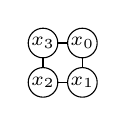
\begin{tikzpicture}[baseline=-2ex, scale=0.5, every node/.style={circle, draw, inner sep=0.5pt, font=\scriptsize}]
    \node (0) at (0,0) {$x_{0}$};
    \node (1) at (0,-1) {$x_{1}$};
    \node (2) at (-1,-1) {$x_{2}$};
    \node (3) at (-1,0) {$x_{3}$};
        \draw (0) -- (1) -- (2) -- (3) -- (0);
\end{tikzpicture}\mid x_{1},x_{2},x_{3},x_{4}\in [n]
\right\}$ and $G=D_{4}=\{e,r,r^{2},r^{3},F,Fr,Fr^{2},Fr^{3}\}.$



The group $D_4$ is isomorphic to the following subgroup of $S_{4}$:
\[
D_4=\{(1)(2)(3)(4),(1234),(13)(24),(1432),(24)(1)(3),(12)(34),(13)(2)(4),(14)(23)\}.
\]
We calculate the size of $|\Fix{}{g}|$ by counting the number of elements (tuples in $[n]^{4}$) of $X$ fixed by $g$, whose general form is given in the second column.
Observe.
\[
\begin{array}{c|c|c}
g & Fix(g)-\text{elements} & |\mathrm{Fix}(g)|\\
\hline
(1)(2)(3)(4) & 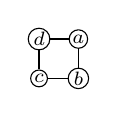
\begin{tikzpicture}[baseline=-2ex, scale=0.5, every node/.style={circle, draw, inner sep=0.5pt, font=\scriptsize}]
    \node (0) at (0,0) {$a$};
    \node (1) at (0,-1) {$b$};
    \node (2) at (-1,-1) {$c$};
    \node (3) at (-1,0) {$d$};
        \draw (0) -- (1) -- (2) -- (3) -- (0);
\end{tikzpicture} & n^4\\
(1234) & 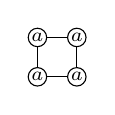
\begin{tikzpicture}[baseline=-2ex, scale=0.5, every node/.style={circle, draw, inner sep=0.5pt, font=\scriptsize}]
    \node (0) at (0,0) {$a$};
    \node (1) at (0,-1) {$a$};
    \node (2) at (-1,-1) {$a$};
    \node (3) at (-1,0) {$a$};
        \draw (0) -- (1) -- (2) -- (3) -- (0);
\end{tikzpicture} & n\\
(13)(24) & 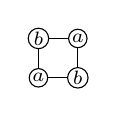
\begin{tikzpicture}[baseline=-2ex, scale=0.5, every node/.style={circle, draw, inner sep=0.5pt, font=\scriptsize}]
    \node (0) at (0,0) {$a$};
    \node (1) at (0,-1) {$b$};
    \node (2) at (-1,-1) {$a$};
    \node (3) at (-1,0) {$b$};
        \draw (0) -- (1) -- (2) -- (3) -- (0);
\end{tikzpicture} & n^2\\
(1432) & 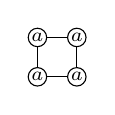
\begin{tikzpicture}[baseline=-2ex, scale=0.5, every node/.style={circle, draw, inner sep=0.5pt, font=\scriptsize}]
    \node (0) at (0,0) {$a$};
    \node (1) at (0,-1) {$a$};
    \node (2) at (-1,-1) {$a$};
    \node (3) at (-1,0) {$a$};
        \draw (0) -- (1) -- (2) -- (3) -- (0);
\end{tikzpicture} & n\\
(24)(1)(3) & 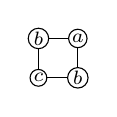
\begin{tikzpicture}[baseline=-2ex, scale=0.5, every node/.style={circle, draw, inner sep=0.5pt, font=\scriptsize}]
    \node (0) at (0,0) {$a$};
    \node (1) at (0,-1) {$b$};
    \node (2) at (-1,-1) {$c$};
    \node (3) at (-1,0) {$b$};
        \draw (0) -- (1) -- (2) -- (3) -- (0);
\end{tikzpicture} & r^3\\
(12)(34) & 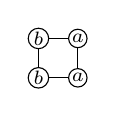
\begin{tikzpicture}[baseline=-2ex, scale=0.5, every node/.style={circle, draw, inner sep=0.5pt, font=\scriptsize}]
    \node (0) at (0,0) {$a$};
    \node (1) at (0,-1) {$a$};
    \node (2) at (-1,-1) {$b$};
    \node (3) at (-1,0) {$b$};
        \draw (0) -- (1) -- (2) -- (3) -- (0);
\end{tikzpicture} & r^2\\
(13)(2)(4) & 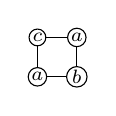
\begin{tikzpicture}[baseline=-2ex, scale=0.5, every node/.style={circle, draw, inner sep=0.5pt, font=\scriptsize}]
    \node (0) at (0,0) {$a$};
    \node (1) at (0,-1) {$b$};
    \node (2) at (-1,-1) {$a$};
    \node (3) at (-1,0) {$c$};
        \draw (0) -- (1) -- (2) -- (3) -- (0);
\end{tikzpicture} & r^3\\
(14)(23) & 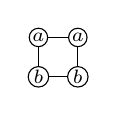
\begin{tikzpicture}[baseline=-2ex, scale=0.5, every node/.style={circle, draw, inner sep=0.5pt, font=\scriptsize}]
    \node (0) at (0,0) {$a$};
    \node (1) at (0,-1) {$b$};
    \node (2) at (-1,-1) {$b$};
    \node (3) at (-1,0) {$a$};
        \draw (0) -- (1) -- (2) -- (3) -- (0);
\end{tikzpicture} & r^2
\end{array}
\]

Thus,
\[
\#(\text{different n-color 4-necklaces up to $D_{4}$})
=\#(\text{distinct $(D_{4}\curvearrowright X)$-orbits})=\frac18\left(n^4+2n^3+3n^2+2n\right).
\]
\end{proof}
%%%%%%%%%%%%%%%%%%%%%%%%%%%%%%%%%%%%%%%%%%%%%%%%%%%%%%%%%%%% 9(a) %%%%%%%%%%%%%%%%%%%%%%%%%%%%%%%%%%%%%%%%%%%%%%%%%%%
\newpage
\setcounter{thm}{8}
\renewcommand{\thethm}{\arabic{thm}(a)}
% Sets the counter to 9(a)
\begin{prob}
Find the number of distinct edge $n$-colorings of a cube under rotations using Burnside's Lemma.
\end{prob}

\begin{proof}
Let $X$ be the set of all edge $n$-colorings of the edges of a cube $X \longleftrightarrow [n]^{12}$ and $G$ be the rotational symmetries of $X$. $S_{4}$ permutes the set of $4$ diagonal poles inside a cube, and those permutations describe rotations of the cube. So these are the same permutations; $G\cong S_{4}.$ The edge labels, vertices, and corresponding poles are shown below:

\begin{center}
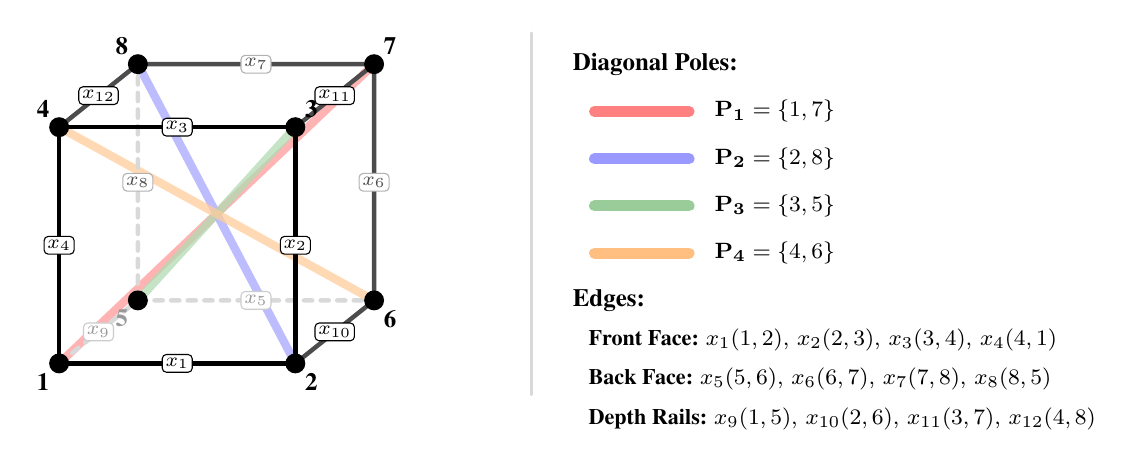
\begin{tikzpicture}[scale=2.0, line join=round, line cap=round, >=stealth]
  % ========================================================
  % 0. COORDINATE DEFINITIONS FOR THE CUBE (Left Side)
  % ========================================================
  % Front face vertices (1, 2, 3, 4)
  \coordinate (V1) at (0,0); 
  \coordinate (V2) at (1.5,0); 
  \coordinate (V3) at (1.5,1.5); 
  \coordinate (V4) at (0,1.5);
  
  % Back face vertices (5, 6, 7, 8)
  \coordinate (V5) at (0.5,0.4); 
  \coordinate (V6) at (2.0,0.4); 
  \coordinate (V7) at (2.0,1.9); 
  \coordinate (V8) at (0.5,1.9);

  % ========================================================
  % 1. DRAW HIGH-CONTRAST DIAGONAL POLES INSIDE CUBE
  % ========================================================
  \draw[line width=3pt, red!40, opacity=0.75] (V1) -- (V7);         % P1
  \draw[line width=3pt, blue!35, opacity=0.75] (V2) -- (V8);        % P2
  \draw[line width=3pt, green!50!black!30, opacity=0.75] (V3) -- (V5); % P3
  \draw[line width=3pt, orange!40, opacity=0.75] (V4) -- (V6);      % P4

  % ========================================================
  % 2. DRAW CUBE WIREFRAME SKELETON
  % ========================================================
  \draw[ultra thick, gray!30, dashed] (V5)--(V6) (V5)--(V8) (V1)--(V5);
  \draw[ultra thick, black!70] (V6)--(V7)--(V8) (V2)--(V6) (V3)--(V7) (V4)--(V8);
  \draw[ultra thick, black] (V1)--(V2)--(V3)--(V4)--cycle;

  % ========================================================
  % 3. LABEL VERTICES (1 through 8)
  % ========================================================
  \fill[black] (V1) circle (1.8pt) node[below left, font=\bfseries\small] {1};
  \fill[black] (V2) circle (1.8pt) node[below right, font=\bfseries\small] {2};
  \fill[black] (V3) circle (1.8pt) node[above right, font=\bfseries\small] {3};
  \fill[black] (V4) circle (1.8pt) node[above left, font=\bfseries\small] {4};
  \fill[black] (V5) circle (1.8pt) node[below left, gray!80, font=\bfseries\small] {5};
  \fill[black] (V6) circle (1.8pt) node[below right, font=\bfseries\small] {6};
  \fill[black] (V7) circle (1.8pt) node[above right, font=\bfseries\small] {7};
  \fill[black] (V8) circle (1.8pt) node[above left, font=\bfseries\small] {8};

  % ========================================================
  % 4. LABEL EDGES (x_1 through x_12) WITH WHITE PILLS
  % ========================================================
  \node[fill=white, draw=black, font=\scriptsize\bfseries, inner sep=1.2pt, rounded corners=1.5pt] at (0.75,0) {$x_1$};
  \node[fill=white, draw=black, font=\scriptsize\bfseries, inner sep=1.2pt, rounded corners=1.5pt] at (1.5,0.75) {$x_2$};
  \node[fill=white, draw=black, font=\scriptsize\bfseries, inner sep=1.2pt, rounded corners=1.5pt] at (0.75,1.5) {$x_3$};
  \node[fill=white, draw=black, font=\scriptsize\bfseries, inner sep=1.2pt, rounded corners=1.5pt] at (0,0.75) {$x_4$};

  \node[fill=white, draw=gray!40, text=gray!80, font=\scriptsize\bfseries, inner sep=1.2pt, rounded corners=1.5pt] at (1.25,0.4) {$x_5$};
  \node[fill=white, draw=gray!60, text=black!70, font=\scriptsize\bfseries, inner sep=1.2pt, rounded corners=1.5pt] at (2.0,1.15) {$x_6$};
  \node[fill=white, draw=gray!60, text=black!70, font=\scriptsize\bfseries, inner sep=1.2pt, rounded corners=1.5pt] at (1.25,1.9) {$x_7$};
  \node[fill=white, draw=gray!60, text=black!70, font=\scriptsize\bfseries, inner sep=1.2pt, rounded corners=1.5pt] at (0.5,1.15) {$x_8$};

  \node[fill=white, draw=gray!40, text=gray!80, font=\scriptsize\bfseries, inner sep=1.2pt, rounded corners=1.5pt] at (0.25,0.2) {$x_9$};
  \node[fill=white, draw=black, font=\scriptsize\bfseries, inner sep=1.2pt, rounded corners=1.5pt] at (1.75,0.2) {$x_{10}$};
  \node[fill=white, draw=black, font=\scriptsize\bfseries, inner sep=1.2pt, rounded corners=1.5pt] at (1.75,1.7) {$x_{11}$};
  \node[fill=white, draw=black, font=\scriptsize\bfseries, inner sep=1.2pt, rounded corners=1.5pt] at (0.25,1.7) {$x_{12}$};

  % ========================================================
  % 5. COLOR-CODED VISUAL KEY (Right Side)
  % ========================================================
  % Structural Divider Line
  \draw[thick, gray!30] (3.0,-0.2) -- (3.0,2.1);

  % POLES SECTION KEY
  \node[anchor=west, font=\bfseries\small] at (3.2,1.9) {Diagonal Poles:};
  
  \draw[line width=4pt, red!50] (3.4,1.6) -- (4.0,1.6);
  \node[anchor=west, font=\footnotesize] at (4.1,1.6) {$\mathbf{P_1} = \{1, 7\}$};

  \draw[line width=4pt, blue!40] (3.4,1.3) -- (4.0,1.3);
  \node[anchor=west, font=\footnotesize] at (4.1,1.3) {$\mathbf{P_2} = \{2, 8\}$};

  \draw[line width=4pt, green!50!black!40] (3.4,1.0) -- (4.0,1.0);
  \node[anchor=west, font=\footnotesize] at (4.1,1.0) {$\mathbf{P_3} = \{3, 5\}$};

  \draw[line width=4pt, orange!50] (3.4,0.7) -- (4.0,0.7);
  \node[anchor=west, font=\footnotesize] at (4.1,0.7) {$\mathbf{P_4} = \{4, 6\}$};

  % EDGES SECTION KEY
  \node[anchor=west, font=\bfseries\small] at (3.2,0.4) {Edges:};
  
  \node[anchor=west, font=\footnotesize] at (3.3,0.15) {\textbf{Front Face:} $x_1(1,2),\, x_2(2,3),\, x_3(3,4),\, x_4(4,1)$};
  \node[anchor=west, font=\footnotesize] at (3.3,-0.1) {\textbf{Back Face:} $x_5(5,6),\, x_6(6,7),\, x_7(7,8),\, x_8(8,5)$};
  \node[anchor=west, font=\footnotesize] at (3.3,-0.35) {\textbf{Depth Rails:} $x_9(1,5),\, x_{10}(2,6),\, x_{11}(3,7),\, x_{12}(4,8)$};

\end{tikzpicture}
\end{center}

So we can just map the action of $S_{4}$ on the poles to permutations of vertices, which we can then map to permutations on edges $X$. We then obtain $c(g)$ via this isomorphism $s\in S_{4}\leftrightarrow v\in V\leftrightarrow g\in G$. Visually this is very simple and we show an example below.

\begin{center}
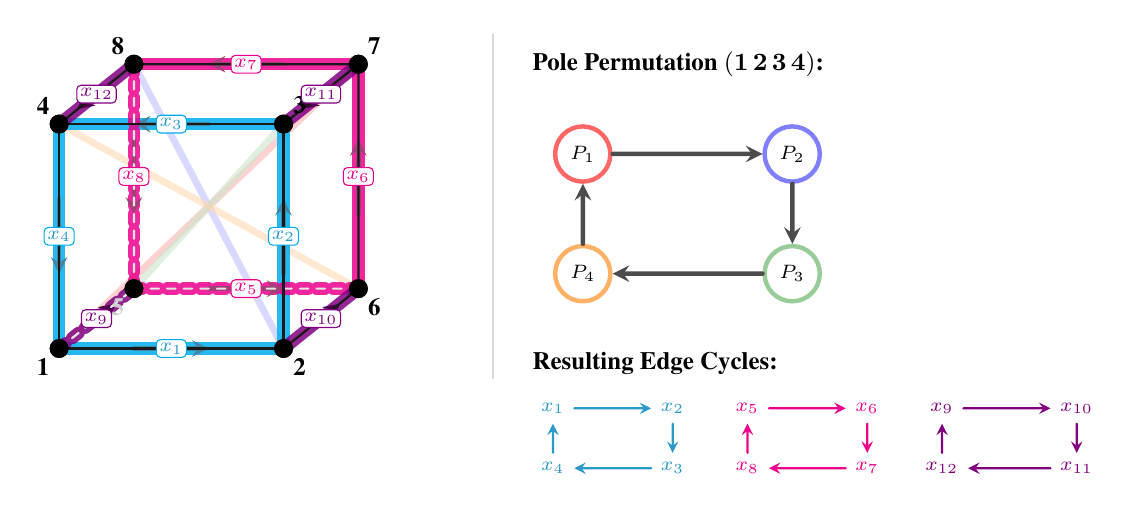
\begin{tikzpicture}[scale=1.9, line join=round, line cap=round, >=stealth]
  % ========================================================
  % 0. COORDINATE DEFINITIONS FOR THE CUBE (Left)
  % ========================================================
  \coordinate (V1) at (0,0); \coordinate (V2) at (1.5,0); \coordinate (V3) at (1.5,1.5); \coordinate (V4) at (0,1.5);
  \coordinate (V5) at (0.5,0.4); \coordinate (V6) at (2.0,0.4); \coordinate (V7) at (2.0,1.9); \coordinate (V8) at (0.5,1.9);

  % ========================================================
  % 1. DRAW INTERNAL DIAGONAL POLES
  % ========================================================
  \draw[line width=2.5pt, red!30, opacity=0.6] (V1) -- (V7);         
  \draw[line width=2.5pt, blue!25, opacity=0.6] (V2) -- (V8);        
  \draw[line width=2.5pt, green!50!black!20, opacity=0.6] (V3) -- (V5); 
  \draw[line width=2.5pt, orange!30, opacity=0.6] (V4) -- (V6);      

  % ========================================================
  % 2. WIREFRAME COLOR OVERLAYS WITH DIRECTIONAL ARROWS
  % ========================================================
  % CYAN TRACK: Front Face Edges (x1, x2, x3, x4)
  \draw[line width=4.5pt, cyan, opacity=0.85] (V1)--(V2)--(V3)--(V4)--cycle;
  \draw[->, ultra thick, cyan!60!black] (0.5,0) -- (1.0,0);
  \draw[->, ultra thick, cyan!60!black] (1.5,0.5) -- (1.5,1.0);
  \draw[->, ultra thick, cyan!60!black] (1.0,1.5) -- (0.5,1.5);
  \draw[->, ultra thick, cyan!60!black] (0,1.0) -- (0,0.5);

  % MAGENTA TRACK: Back Face Edges (x5, x6, x7, x8)
  \draw[line width=4.5pt, magenta, opacity=0.85, dashed] (V5)--(V6) (V5)--(V8);
  \draw[line width=4.5pt, magenta, opacity=0.85] (V6)--(V7)--(V8);
  \draw[->, ultra thick, magenta!60!black] (1.0,0.4) -- (1.5,0.4);
  \draw[->, ultra thick, magenta!60!black] (2.0,0.9) -- (2.0,1.4);
  \draw[->, ultra thick, magenta!60!black] (1.5,1.9) -- (1.0,1.9);
  \draw[->, ultra thick, magenta!60!black, dashed] (0.5,1.4) -- (0.5,0.9);

  % VIOLET TRACK: Connecting Depth Rails (x9, x10, x11, x12)
  \draw[line width=4.5pt, violet, opacity=0.85, dashed] (V1)--(V5); 
  \draw[line width=4.5pt, violet, opacity=0.85] (V2)--(V6) (V3)--(V7) (V4)--(V8);
  \draw[->, ultra thick, violet!60!black, dashed] (0.25,0.2) -- (0.38,0.3);
  \draw[->, ultra thick, violet!60!black] (1.75,0.2) -- (1.88,0.3);
  \draw[->, ultra thick, violet!60!black] (1.75,1.7) -- (1.62,1.6);
  \draw[->, ultra thick, violet!60!black] (0.25,1.7) -- (0.12,1.6);

  % ========================================================
  % 3. CHASSIS OUTLINES (Thin sharp lines on top)
  % ========================================================
  \draw[thick, gray!20, dashed] (V5)--(V6) (V5)--(V8) (V1)--(V5);
  \draw[thick, black!90] (V6)--(V7)--(V8) (V2)--(V6) (V3)--(V7) (V4)--(V8);
  \draw[thick, black!90] (V1)--(V2)--(V3)--(V4)--cycle;

  % Vertex Anchors
  \foreach \v in {V1,V2,V3,V4,V5,V6,V7,V8} \fill[black] (\v) circle (1.8pt);
  \fill[black] (V1) circle (1.8pt) node[below left, font=\bfseries\small] {1};
  \fill[black] (V2) circle (1.8pt) node[below right, font=\bfseries\small] {2};
  \fill[black] (V3) circle (1.8pt) node[above right, font=\bfseries\small] {3};
  \fill[black] (V4) circle (1.8pt) node[above left, font=\bfseries\small] {4};
  \fill[black] (V5) circle (1.8pt) node[below left, gray!40, font=\bfseries\small] {5};
  \fill[black] (V6) circle (1.8pt) node[below right, font=\bfseries\small] {6};
  \fill[black] (V7) circle (1.8pt) node[above right, font=\bfseries\small] {7};
  \fill[black] (V8) circle (1.8pt) node[above left, font=\bfseries\small] {8};

  % Edge Pill Labels
  \node[fill=white, draw=cyan, text=cyan!80!black, font=\scriptsize\bfseries, inner sep=1.2pt, rounded corners=1.5pt] at (0.75,0) {$x_1$};
  \node[fill=white, draw=cyan, text=cyan!80!black, font=\scriptsize\bfseries, inner sep=1.2pt, rounded corners=1.5pt] at (1.5,0.75) {$x_2$};
  \node[fill=white, draw=cyan, text=cyan!80!black, font=\scriptsize\bfseries, inner sep=1.2pt, rounded corners=1.5pt] at (0.75,1.5) {$x_3$};
  \node[fill=white, draw=cyan, text=cyan!80!black, font=\scriptsize\bfseries, inner sep=1.2pt, rounded corners=1.5pt] at (0,0.75) {$x_4$};

  \node[fill=white, draw=magenta, text=magenta, font=\scriptsize\bfseries, inner sep=1.2pt, rounded corners=1.5pt] at (1.25,0.4) {$x_5$};
  \node[fill=white, draw=magenta, text=magenta, font=\scriptsize\bfseries, inner sep=1.2pt, rounded corners=1.5pt] at (2.0,1.15) {$x_6$};
  \node[fill=white, draw=magenta, text=magenta, font=\scriptsize\bfseries, inner sep=1.2pt, rounded corners=1.5pt] at (1.25,1.9) {$x_7$};
  \node[fill=white, draw=magenta, text=magenta, font=\scriptsize\bfseries, inner sep=1.2pt, rounded corners=1.5pt] at (0.5,1.15) {$x_8$};

  \node[fill=white, draw=violet, text=violet, font=\scriptsize\bfseries, inner sep=1.2pt, rounded corners=1.5pt] at (0.25,0.2) {$x_9$};
  \node[fill=white, draw=violet, text=violet, font=\scriptsize\bfseries, inner sep=1.2pt, rounded corners=1.5pt] at (1.75,0.2) {$x_{10}$};
  \node[fill=white, draw=violet, text=violet, font=\scriptsize\bfseries, inner sep=1.2pt, rounded corners=1.5pt] at (1.75,1.7) {$x_{11}$};
  \node[fill=white, draw=violet, text=violet, font=\scriptsize\bfseries, inner sep=1.2pt, rounded corners=1.5pt] at (0.25,1.7) {$x_{12}$};

  % ========================================================
  % 5. POLE PERMUTATION ARROW NETWORK (Right Side)
  % ========================================================
  \draw[thick, gray!30] (2.9,-0.2) -- (2.9,2.1);

  \node[anchor=west, font=\bfseries\small] at (3.1,1.9) {Pole Permutation $\mathbf{(1\,2\,3\,4)}$:};

  % Position the 4 pole stations with matching line colors
  \node (N1) at (3.5,1.3) [draw=red!60, fill=white, ultra thick, circle, font=\scriptsize\bfseries] {$P_1$};
  \node (N2) at (4.9,1.3) [draw=blue!50, fill=white, ultra thick, circle, font=\scriptsize\bfseries] {$P_2$};
  \node (N3) at (4.9,0.5) [draw=green!50!black!40, fill=white, ultra thick, circle, font=\scriptsize\bfseries] {$P_3$};
  \node (N4) at (3.5,0.5) [draw=orange!60, fill=white, ultra thick, circle, font=\scriptsize\bfseries] {$P_4$};

  % Connecting structural permutation arrows
  \draw[->, ultra thick, black!70] (N1) -- (N2);
  \draw[->, ultra thick, black!70] (N2) -- (N3);
  \draw[->, ultra thick, black!70] (N3) -- (N4);
  \draw[->, ultra thick, black!70] (N4) -- (N1);

  % Edge Loops matching the respective track profiles
  \node[anchor=west, font=\bfseries\small] at (3.1,-0.1) {Resulting Edge Cycles:};

  % Front Face Loop
  \node (X1) at (3.3,-0.4)  [font=\scriptsize\bfseries, text=cyan!80!black] {$x_1$};
  \node (X2) at (4.1,-0.4)  [font=\scriptsize\bfseries, text=cyan!80!black] {$x_2$};
  \node (X3) at (4.1,-0.8)  [font=\scriptsize\bfseries, text=cyan!80!black] {$x_3$};
  \node (X4) at (3.3,-0.8)  [font=\scriptsize\bfseries, text=cyan!80!black] {$x_4$};
  \draw[->, thick, cyan!80!black] (X1) -- (X2); \draw[->, thick, cyan!80!black] (X2) -- (X3);
  \draw[->, thick, cyan!80!black] (X3) -- (X4); \draw[->, thick, cyan!80!black] (X4) -- (X1);

  % Back Face Loop
  \node (X5) at (4.6,-0.4)  [font=\scriptsize\bfseries, text=magenta] {$x_5$};
  \node (X6) at (5.4,-0.4)  [font=\scriptsize\bfseries, text=magenta] {$x_6$};
  \node (X7) at (5.4,-0.8)  [font=\scriptsize\bfseries, text=magenta] {$x_7$};
  \node (X8) at (4.6,-0.8)  [font=\scriptsize\bfseries, text=magenta] {$x_8$};
  \draw[->, thick, magenta] (X5) -- (X6); \draw[->, thick, magenta] (X6) -- (X7);
  \draw[->, thick, magenta] (X7) -- (X8); \draw[->, thick, magenta] (X8) -- (X5);

  % Depth Rails Loop
  \node (X9) at (5.9,-0.4)  [font=\scriptsize\bfseries, text=violet] {$x_9$};
  \node (X10) at (6.8,-0.4) [font=\scriptsize\bfseries, text=violet] {$x_{10}$};
  \node (X11) at (6.8,-0.8) [font=\scriptsize\bfseries, text=violet] {$x_{11}$};
  \node (X12) at (5.9,-0.8) [font=\scriptsize\bfseries, text=violet] {$x_{12}$};
  \draw[->, thick, violet] (X9) -- (X10); \draw[->, thick, violet] (X10) -- (X11);
  \draw[->, thick, violet] (X11) -- (X12); \draw[->, thick, violet] (X12) -- (X9);

\end{tikzpicture}
\end{center}

So $c(g)=3$ as shown from the resulting edge cycles, and then $|\Fix{}{g}|=n^(c(g))=n^3$. We show the rest of the computations below.

\noindent 
\bgroup
\def\arraystretch{1} 
\begin{center}
\begin{tabular}{l|l|c|c}
\textbf{Geometric Rotation Class} & \textbf{Pole Permutation $g \in S_4$} & $c(g)$ & $|\mathrm{Fix}(g)|$ \\
\hline
\textbf{1) Identity (1 element)} & & & \\
Identity & $(1)(2)(3)(4)$ & 12 & $n^{12}$ \\
\hline
\textbf{2) Face-Center Rotations (9 elements)} & & & \\
$90^\circ$ around Z-axis & $(1\,2\,3\,4)$ & 3 & $n^3$ \\
$270^\circ$ around Z-axis & $(1\,4\,3\,2)$ & 3 & $n^3$ \\
$180^\circ$ around Z-axis & $(1\,3)(2\,4)$ & 6 & $n^6$ \\
$90^\circ$ around Y-axis & $(1\,4\,2\,3)$ & 3 & $n^3$ \\
$270^\circ$ around Y-axis & $(1\,3\,2\,4)$ & 3 & $n^3$ \\
$180^\circ$ around Y-axis & $(1\,2)(3\,4)$ & 6 & $n^6$ \\
$90^\circ$ around X-axis & $(1\,3\,4\,2)$ & 3 & $n^3$ \\
$270^\circ$ around X-axis & $(1\,2\,4\,3)$ & 3 & $n^3$ \\
$180^\circ$ around X-axis & $(1\,4)(2\,3)$ & 6 & $n^6$ \\
\hline
\textbf{3) Edge-Center $180^\circ$ Flips (6 elements)} & & & \\
Flip via $x_1/x_7$ midpoint & $(1\,2)(3)(4)$ & 7 & $n^7$ \\
Flip via $x_3/x_5$ midpoint & $(3\,4)(1)(2)$ & 7 & $n^7$ \\
Flip via $x_2/x_8$ midpoint & $(1\,3)(2)(4)$ & 7 & $n^7$ \\
Flip via $x_4/x_6$ midpoint & $(2\,4)(1)(3)$ & 7 & $n^7$ \\
Flip via $x_9/x_{11}$ midpoint & $(1\,4)(2)(3)$ & 7 & $n^7$ \\
Flip via $x_{10}/x_{12}$ midpoint & $(2\,3)(1)(4)$ & 7 & $n^7$ \\
\hline
\textbf{4) Vertex-Center $120^\circ/240^\circ$ Spins (8 elements)} & & & \\
$120^\circ$ spin around Pole $P_1$ & $(1)(2\,3\,4)$ & 4 & $n^4$ \\
$240^\circ$ spin around Pole $P_1$ & $(1)(2\,4\,3)$ & 4 & $n^4$ \\
$120^\circ$ spin around Pole $P_2$ & $(2)(1\,4\,3)$ & 4 & $n^4$ \\
$240^\circ$ spin around Pole $P_2$ & $(2)(1\,3\,4)$ & 4 & $n^4$ \\
$120^\circ$ spin around Pole $P_3$ & $(3)(1\,2\,4)$ & 4 & $n^4$ \\
$240^\circ$ spin around Pole $P_3$ & $(3)(1\,4\,2)$ & 4 & $n^4$ \\
$120^\circ$ spin around Pole $P_4$ & $(4)(1\,3\,2)$ & 4 & $n^4$ \\
$240^\circ$ spin around Pole $P_4$ & $(4)(1\,2\,3)$ & 4 & $n^4$ \\
\end{tabular}
\end{center}
\egroup

\noindent By Burnside's Lemma, we average the number of fixed configurations across the 24 pole permutations of $S_4$:
\[
\#(\text{distinct edge } n\text{-colorings}) = \#(\text{distinct $(G\curvearrowright X)$-orbits})= \frac{1}{|S_{4}|}\sum_{g\in S_4}|\mathrm{Fix}(g)|
\]
Adding all $n$-polynomials in the last row of the table we get the following
\[
\#(\text{distinct edge $n$-colorings}) = \frac{1}{24}\left(n^{12} + 3n^6 + 6n^7 + 8n^4 + 6n^3\right)
\]

\end{proof}


%%%%%%%%%%%%%%%%%%%%%%%%%%%%%%%%%%%%%%%%%%%%%%%%%%%%%%%%%%%% 11 (b) %%%%%%%%%%%%%%%%%%%%%%%%%%%%%%%%%%%%%%%%%%%%%%%%%%%
\newpage
\setcounter{thm}{10}
\renewcommand{\thethm}{\arabic{thm}(a)}

\begin{prob}
Compute the cycle index polynomial for $\langle (1\cdots n)\rangle \cong Z_{n}\curvearrowright X= [n].$
\end{prob}
\begin{proof} Recall: For a finite group $G$ acting on a finite set $X$ with $|X|=n$, the cycle index polynomial is

\[
Z(G \curvearrowright X)
=
\frac{1}{|G|}
\sum_{g\in G}
\prod_{i=1}^{n} a_i^{c_i(g)},
\]

Let $\sigma = (1\,2\,\dots\,n)\implies G=\langle \sigma\rangle \cong Z_{n}$ once more. We determine the cycle structure of $\sigma^k$ permuting $[n]$ for each $k=1,\hdots, n$.

Take $[n]$ to be $\mathbb{Z}_n$. Then, to compute the length of any cycle in the 'maximal length decomposition' of $\sigma^{k}$, fix $i\in [n]$ and apply $\sigma^{k}$ repeatedly to see in how many steps it wraps back to itself; to see how long the cycle it is contained in is.
\[
\sigma^{k}(i)=i+k\pmod n\implies (\sigma^{k})^{j}(i)=i\text{ when }i+jk\equiv i\pmod n\iff jk\equiv 0\pmod n. 
\]

So we see that for any $i$, the cycle length is the minimal number $j$ such that $jk\equiv \pmod n;|k|_{\ZZ_{n}}$, which is not only well-known to be $|k|_{\ZZ_{n}}=\frac{n}{\gcd(k,n)}$ but it is also independent of which $i\in [n]$ being permuted. So $\sigma^{k}$ must partition $[n]$ into $m=\frac{n}{\frac{n}{\gcd(k,n)}}=\gcd(n,k)$ equal parts of length $\frac{n}{\gcd(k,n)}$. In more precise terms, $\sigma^{k}$ decomposes into exactly $\gcd(n,k)$ cycles which all have length $\frac{n}{\gcd(n,k)}$. That is,

\[
\sigma^{k}\text{ contributes }a_{\frac{n}{\gcd(k,n)}}^{\gcd(n,k)}=a_{|k|_{\ZZ_{n}}}^{\gcd(n,k)}\text{ to the cycle index polynomial of }G\curvearrowright [n].
\]

Well, by Lagrange the only possible orders in $G\cong \ZZ_{n}$ are divisors $d$ of $n$, in terms of $d=|k|_{\ZZ_{n}}=\frac{n}{\gcd(n,k)}$, we will have that $gcd(n,k)=\frac{n}{d}\implies a_{|k|_{\ZZ_{n}}}^{\gcd(n,k)}=a_{d}^{\frac{n}{d}}$. Finally, since $G$ is cyclic of order $n$, there are exactly $\varphi(d)$ elements of order $d$ for each divisor $d$ of $n$. So we can just sum over divisors of $n$ to obtain:
$$
Z(G;a_{1},\hdots,a_{n})
=\frac{1}{|G|}
\sum_{g\in G}
\prod_{i=1}^{n} a_i^{c_i(g)}=Z(\ZZ_{n}; a_{1},\hdots,a_{n})
=\frac{1}{n}
\sum_{k\in \ZZ_{n}}
a_{|k|_{\ZZ_{n}}}^{\gcd(k,n)}=\frac{1}{n}
\sum_{d\mid n}
\varphi(d) a_d^{\frac{n}{d}}.
$$
\end{proof}

%%%%%%%%%%%%%%%%%%%%%%%%%%%%%%%%%%%%%%%%%%%%%%%%%%%%%%%%%%%% 11 (c) %%%%%%%%%%%%%%%%%%%%%%%%%%%%%%%%%%%%%%%%%%%%%%%%%%%
\newpage
\setcounter{thm}{10}
\renewcommand{\thethm}{\arabic{thm}(a)}

\begin{prob}
Compute the cycle index polynomial for the rotational symmetries of the cube acting on faces.
\end{prob}

\begin{proof}
Let $X$ be the set of faces of a cube, so $X\longleftrightarrow [6]$, and let $G$ be the group of rotational symmetries of the cube, which we established is $S_{4}$ in the previous problem. Once more we can just define a correspondence between that action on the poles, vertices, and then faces to compute everything.
\usetikzlibrary{calc}
\begin{center}
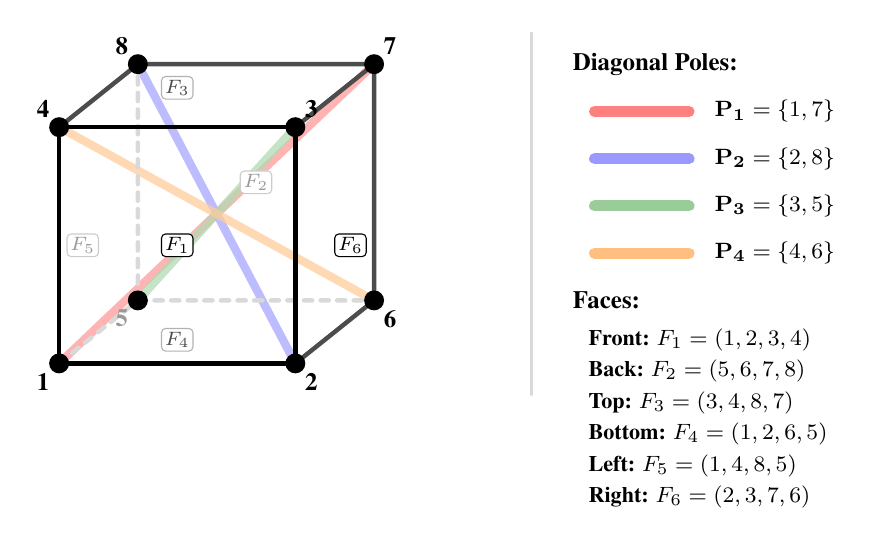
\begin{tikzpicture}[scale=2.0, line join=round, line cap=round, >=stealth]
  % ========================================================
  % 0. COORDINATE DEFINITIONS FOR THE CUBE (Left Side)
  % ========================================================
  % Front face vertices (1, 2, 3, 4)
  \coordinate (V1) at (0,0); 
  \coordinate (V2) at (1.5,0); 
  \coordinate (V3) at (1.5,1.5); 
  \coordinate (V4) at (0,1.5);
  
  % Back face vertices (5, 6, 7, 8)
  \coordinate (V5) at (0.5,0.4); 
  \coordinate (V6) at (2.0,0.4); 
  \coordinate (V7) at (2.0,1.9); 
  \coordinate (V8) at (0.5,1.9);

  % ========================================================
  % 1. DRAW HIGH-CONTRAST DIAGONAL POLES INSIDE CUBE (colored)
  % ========================================================
  \draw[line width=3pt, red!40, opacity=0.75] (V1) -- (V7);         % P1
  \draw[line width=3pt, blue!35, opacity=0.75] (V2) -- (V8);        % P2
  \draw[line width=3pt, green!50!black!30, opacity=0.75] (V3) -- (V5); % P3
  \draw[line width=3pt, orange!40, opacity=0.75] (V4) -- (V6);      % P4

  % ========================================================
  % 2. DRAW CUBE WIREFRAME SKELETON (unchanged)
  % ========================================================
  \draw[ultra thick, gray!30, dashed] (V5)--(V6) (V5)--(V8) (V1)--(V5);
  \draw[ultra thick, black!70] (V6)--(V7)--(V8) (V2)--(V6) (V3)--(V7) (V4)--(V8);
  \draw[ultra thick, black] (V1)--(V2)--(V3)--(V4)--cycle;

  % ========================================================
  % 3. LABEL VERTICES (1 through 8)
  % ========================================================
  \fill[black] (V1) circle (1.8pt) node[below left, font=\bfseries\small] {1};
  \fill[black] (V2) circle (1.8pt) node[below right, font=\bfseries\small] {2};
  \fill[black] (V3) circle (1.8pt) node[above right, font=\bfseries\small] {3};
  \fill[black] (V4) circle (1.8pt) node[above left, font=\bfseries\small] {4};
  \fill[black] (V5) circle (1.8pt) node[below left, gray!80, font=\bfseries\small] {5};
  \fill[black] (V6) circle (1.8pt) node[below right, font=\bfseries\small] {6};
  \fill[black] (V7) circle (1.8pt) node[above right, font=\bfseries\small] {7};
  \fill[black] (V8) circle (1.8pt) node[above left, font=\bfseries\small] {8};

  % ========================================================
  % 4. LABEL FACES (F1 through F6) placed to match original edge positions
  % ========================================================
  % Front face (vertices 1,2,3,4)
  \node[fill=white, draw=black, font=\scriptsize\bfseries, inner sep=1.2pt, rounded corners=1.5pt] at (0.75,0.75) {$F_1$};

  % Back face (vertices 5,6,7,8)
  \node[fill=white, draw=gray!40, text=gray!80, font=\scriptsize\bfseries, inner sep=1.2pt, rounded corners=1.5pt] at (1.25,1.15) {$F_2$};

  % Top face (vertices 3,4,8,7)
  \node[fill=white, draw=gray!60, text=black!70, font=\scriptsize\bfseries, inner sep=1.2pt, rounded corners=1.5pt] at (0.75,1.75) {$F_3$};

  % Bottom face (vertices 1,2,6,5)
  \node[fill=white, draw=gray!60, text=black!70, font=\scriptsize\bfseries, inner sep=1.2pt, rounded corners=1.5pt] at (0.75,0.15) {$F_4$};

  % Left face (vertices 1,4,8,5)
  \node[fill=white, draw=gray!40, text=gray!80, font=\scriptsize\bfseries, inner sep=1.2pt, rounded corners=1.5pt] at (0.15,0.75) {$F_5$};

  % Right face (vertices 2,3,7,6)
  \node[fill=white, draw=black, font=\scriptsize\bfseries, inner sep=1.2pt, rounded corners=1.5pt] at (1.85,0.75) {$F_6$};

  % ========================================================
  % 5. COLOR-CODED VISUAL KEY (Right Side) with Poles and Face Sub-Groups (4-tuples)
  % ========================================================
  % Structural Divider Line
  \draw[thick, gray!30] (3.0,-0.2) -- (3.0,2.1);

  % POLES SECTION KEY
  \node[anchor=west, font=\bfseries\small] at (3.2,1.9) {Diagonal Poles:};
  
  \draw[line width=4pt, red!50] (3.4,1.6) -- (4.0,1.6);
  \node[anchor=west, font=\footnotesize] at (4.1,1.6) {$\mathbf{P_1} = \{1, 7\}$};

  \draw[line width=4pt, blue!40] (3.4,1.3) -- (4.0,1.3);
  \node[anchor=west, font=\footnotesize] at (4.1,1.3) {$\mathbf{P_2} = \{2, 8\}$};

  \draw[line width=4pt, green!50!black!40] (3.4,1.0) -- (4.0,1.0);
  \node[anchor=west, font=\footnotesize] at (4.1,1.0) {$\mathbf{P_3} = \{3, 5\}$};

  \draw[line width=4pt, orange!50] (3.4,0.7) -- (4.0,0.7);
  \node[anchor=west, font=\footnotesize] at (4.1,0.7) {$\mathbf{P_4} = \{4, 6\}$};

  % FACES SECTION KEY (4-tuples)
  \node[anchor=west, font=\bfseries\small] at (3.2,0.4) {Faces:};
  
  \node[anchor=west, font=\footnotesize] at (3.3,0.15) {\textbf{Front:} $F_1 = (1,2,3,4)$};
  \node[anchor=west, font=\footnotesize] at (3.3,-0.05) {\textbf{Back:} $F_2 = (5,6,7,8)$};
  \node[anchor=west, font=\footnotesize] at (3.3,-0.25) {\textbf{Top:} $F_3 = (3,4,8,7)$};
  \node[anchor=west, font=\footnotesize] at (3.3,-0.45) {\textbf{Bottom:} $F_4 = (1,2,6,5)$};
  \node[anchor=west, font=\footnotesize] at (3.3,-0.65) {\textbf{Left:} $F_5 = (1,4,8,5)$};
  \node[anchor=west, font=\footnotesize] at (3.3,-0.85) {\textbf{Right:} $F_6 = (2,3,7,6)$};

\end{tikzpicture}
\end{center}

We show an example below of this correspondence with face permutations

\usetikzlibrary{calc}
\begin{center}
\begin{tikzpicture}[scale=2.0, line join=round, line cap=round, >=stealth]
  % ========================================================
  % 0. COORDINATE DEFINITIONS FOR THE CUBE (Left Side) -- unchanged
  % ========================================================
  % Front face vertices (1, 2, 3, 4)
  \coordinate (V1) at (0,0); 
  \coordinate (V2) at (1.5,0); 
  \coordinate (V3) at (1.5,1.5); 
  \coordinate (V4) at (0,1.5);
  
  % Back face vertices (5, 6, 7, 8)
  \coordinate (V5) at (0.5,0.4); 
  \coordinate (V6) at (2.0,0.4); 
  \coordinate (V7) at (2.0,1.9); 
  \coordinate (V8) at (0.5,1.9);

  % ========================================================
  % 1. DRAW HIGH-CONTRAST DIAGONAL POLES INSIDE CUBE (colored, background only)
  % ========================================================
  \draw[line width=3pt, red!40, opacity=0.75] (V1) -- (V7);         % P1
  \draw[line width=3pt, blue!35, opacity=0.75] (V2) -- (V8);        % P2
  \draw[line width=3pt, green!50!black!30, opacity=0.75] (V3) -- (V5); % P3
  \draw[line width=3pt, orange!40, opacity=0.75] (V4) -- (V6);      % P4

  % ========================================================
  % 2. DRAW CUBE WIREFRAME SKELETON (edges NOT colored)
  % ========================================================
  \draw[ultra thick, gray!30, dashed] (V5)--(V6) (V5)--(V8) (V1)--(V5);
  \draw[ultra thick, black!70] (V6)--(V7)--(V8) (V2)--(V6) (V3)--(V7) (V4)--(V8);
  \draw[ultra thick, black] (V1)--(V2)--(V3)--(V4)--cycle;

  % ========================================================
  % 3. LABEL VERTICES (1 through 8)
  % ========================================================
  \fill[black] (V1) circle (1.8pt) node[below left, font=\bfseries\small] {1};
  \fill[black] (V2) circle (1.8pt) node[below right, font=\bfseries\small] {2};
  \fill[black] (V3) circle (1.8pt) node[above right, font=\bfseries\small] {3};
  \fill[black] (V4) circle (1.8pt) node[above left, font=\bfseries\small] {4};
  \fill[black] (V5) circle (1.8pt) node[below left, gray!80, font=\bfseries\small] {5};
  \fill[black] (V6) circle (1.8pt) node[below right, font=\bfseries\small] {6};
  \fill[black] (V7) circle (1.8pt) node[above right, font=\bfseries\small] {7};
  \fill[black] (V8) circle (1.8pt) node[above left, font=\bfseries\small] {8};

  % ========================================================
  % 4. FACE LABELS (shaded boxes only; left-side identical layout)
  %    - F1: cyan
  %    - F2: its own distinct color (orange)
  %    - F3-F6: same magenta/purple shade
  % ========================================================
  % Front face (F1)
  \node[draw=cyan!70, fill=cyan!12, rounded corners=1.5pt, inner sep=1.2pt, font=\scriptsize\bfseries, text=cyan!80!black] at (0.75,0.75) {$F_1$};

  % Back face (F2) -- its own color
  \node[draw=orange!60, fill=orange!12, rounded corners=1.5pt, inner sep=1.2pt, font=\scriptsize\bfseries, text=orange!60!black] at (1.25,1.15) {$F_2$};

  % Top face (F3) -- group color (magenta/purple)
  \node[draw=magenta!65, fill=magenta!8, rounded corners=1.5pt, inner sep=1.2pt, font=\scriptsize\bfseries, text=magenta!65!black] at (0.75,1.75) {$F_3$};

  % Bottom face (F4) -- group color (magenta/purple)
  \node[draw=magenta!65, fill=magenta!8, rounded corners=1.5pt, inner sep=1.2pt, font=\scriptsize\bfseries, text=magenta!65!black] at (0.75,0.15) {$F_4$};

  % Left face (F5) -- group color (magenta/purple)
  \node[draw=magenta!65, fill=magenta!8, rounded corners=1.5pt, inner sep=1.2pt, font=\scriptsize\bfseries, text=magenta!65!black] at (0.15,0.75) {$F_5$};

  % Right face (F6) -- group color (magenta/purple)
  \node[draw=magenta!65, fill=magenta!8, rounded corners=1.5pt, inner sep=1.2pt, font=\scriptsize\bfseries, text=magenta!65!black] at (1.85,0.75) {$F_6$};

  % ========================================================
  % 5. COLOR-CODED VISUAL KEY (Right Side) with Poles and Face Sub-Groups
  % ========================================================
  % Structural Divider Line (keeps same x-position as your sample)
  \draw[thick, gray!30] (3.0,-0.2) -- (3.0,2.1);

  % ========================================================
  % 6. RIGHT-SIDE: Pole permutation network and resulting face cycles
  %    - Pole permutation block kept identical to your sample
  %    - Face-cycle diagram placed BELOW the "Resulting Face Cycles:" label
  %    - F1: cyan self-loop (loop drawn to the left of the node)
  %    - F2: orange self-loop (loop drawn to the right of the node)
  %    - F3,F6,F5,F4: magenta 4-cycle (all same color) placed below the two self-loops
  % ========================================================

  % Pole permutation header and stations (positions match sample)
  \node[anchor=west, font=\bfseries\small] at (3.1,1.9) {Pole Permutation $\mathbf{(1\,2\,3\,4)}$:};

  \node (N1) at (3.5,1.3) [draw=red!60, fill=white, ultra thick, circle, font=\scriptsize\bfseries] {$P_1$};
  \node (N2) at (4.9,1.3) [draw=blue!50, fill=white, ultra thick, circle, font=\scriptsize\bfseries] {$P_2$};
  \node (N3) at (4.9,0.5) [draw=green!50!black!40, fill=white, ultra thick, circle, font=\scriptsize\bfseries] {$P_3$};
  \node (N4) at (3.5,0.5) [draw=orange!60, fill=white, ultra thick, circle, font=\scriptsize\bfseries] {$P_4$};

  \draw[->, ultra thick, black!70] (N1) -- (N2);
  \draw[->, ultra thick, black!70] (N2) -- (N3);
  \draw[->, ultra thick, black!70] (N3) -- (N4);
  \draw[->, ultra thick, black!70] (N4) -- (N1);

  % Resulting Face Cycles header (flush with pole block)
  \node[anchor=west, font=\bfseries\small] at (3.1,-0.1) {Resulting Face Cycles:};

  % --- place the two self-loop nodes directly below the header (centered under header)
  % F1 node (cyan) with a loop drawn to its left (twirly left-side loop)
  \node (R_F1) at (3.5,-0.35) [draw=cyan!70, fill=cyan!12, rounded corners=1.5pt, inner sep=2pt, font=\scriptsize\bfseries, text=cyan!80!black] {$F_1$};
  \draw[->, thick, cyan!80!black] ($(R_F1.west)+(-0.18,0)$) .. controls ($(R_F1.west)+(-0.9,0.25)$) and ($(R_F1.west)+(-0.9,-0.25)$) .. ($(R_F1.west)+(-0.18,0)$);

  % F2 node (orange) with a loop drawn to its right (twirly right-side loop)
  \node (R_F2) at (4.3,-0.35) [draw=orange!60, fill=orange!12, rounded corners=1.5pt, inner sep=2pt, font=\scriptsize\bfseries, text=orange!60!black] {$F_2$};
  \draw[->, thick, orange!70!black] ($(R_F2.east)+(0.18,0)$) .. controls ($(R_F2.east)+(0.9,0.25)$) and ($(R_F2.east)+(0.9,-0.25)$) .. ($(R_F2.east)+(0.18,0)$);

  % --- 4-cycle (magenta) arranged directly below the two self-loops (2x2 block)
  % ordering chosen to match (F3 F6 F5 F4)
  \node (R_F3) at (3.5,-0.75)  [draw=magenta!60, fill=magenta!12, rounded corners=1.5pt, inner sep=2pt, font=\scriptsize\bfseries] {$F_3$};
  \node (R_F6) at (4.3,-0.75)  [draw=magenta!60, fill=magenta!12, rounded corners=1.5pt, inner sep=2pt, font=\scriptsize\bfseries] {$F_6$};
  \node (R_F5) at (4.3,-1.15)  [draw=magenta!60, fill=magenta!12, rounded corners=1.5pt, inner sep=2pt, font=\scriptsize\bfseries] {$F_5$};
  \node (R_F4) at (3.5,-1.15)  [draw=magenta!60, fill=magenta!12, rounded corners=1.5pt, inner sep=2pt, font=\scriptsize\bfseries] {$F_4$};

  \draw[->, thick, magenta!70!black] (R_F3) -- (R_F6);
  \draw[->, thick, magenta!70!black] (R_F6) -- (R_F5);
  \draw[->, thick, magenta!70!black] (R_F5) -- (R_F4);
  \draw[->, thick, magenta!70!black] (R_F4) -- (R_F3);

\end{tikzpicture}
\end{center}

Recall that the monomial $a_{1}^{c_{1}(g)}a_{2}^{c_{2}(g)}a_{3}^{c_{3}(g)}a_{4}^{c_{4}(g)}a_{5}^{c_{5}(g)}a_{6}^{c_{6}(g)}$ for each $g\in G$ count the number of permutations $g\in G$ that result in $c_{i}$-many $i-$face cycles for each $i\in [4]$. So the cycle index polynomial $Z_{G}$ in general counts the number of permutations $g\in G$ that result in each possible face cycle partition/configuration of $X$. Here we see that $(1234)$ contributes the monomial $a_{1}^{2}a_{4}$.

\medskip
\noindent
\textbf{Rotation classes and face cycle monomials}

\begingroup
\def\arraystretch{1.1}
\begin{center}
\begin{tabular}{l|c|c}
\textbf{Rotation Types} & \textbf{Count} & \textbf{Cycle monomial on faces} \\
\hline
Identity & $1$ & $a_1^6$ \\
\hline
$90^\circ/270^\circ$ about face-center axis & $6$ & $a_1^2 a_4$ \\
\hline
$180^\circ$ about face-center axis & $3$ & $a_1^2 a_2^2$ \\
\hline
$120^\circ/240^\circ$ about body diagonal & $8$ & $a_3^2$ \\
\hline
$180^\circ$ about midpoint of opposite edges & $6$ & $a_2^3$ \\
\end{tabular}
\end{center}
\endgroup
\textbf{Cycle index polynomial}

Summing the right side of the table we get that the cycle index polynomial $Z_{G}$ of $G$ acting on the $6$ faces is


\[
Z_G(a_1,a_2,a_3,a_4,a_5,a_6)
= \frac{1}{|G|} \sum_{g \in G} a_1^{c_1(g)} a_2^{c_2(g)} a_3^{c_3(g)} a_4^{c_4(g)} a_5^{c_5(g)} a_6^{c_6(g)}.
\]


Since $G\cong S_{4}$, we get that 


\[
Z_G(a_1,a_2,a_3,a_4,a_5,a_6)
= \frac{1}{24}\Big(
  a_1^6
  + 6 a_1^2 a_4
  + 3 a_1^2 a_2^2
  + 8 a_3^2
  + 6 a_2^3
\Big).
\]



This is the desired cycle index polynomial for the action of cube rotations on its faces.

\end{proof}

%%%%%%%%%%%%%%%%%%%%%%%%%%%%%%%%%%%%%%%%%%%%%%%%%%%%%%%%%%%% 11 (d) %%%%%%%%%%%%%%%%%%%%%%%%%%%%%%%%%%%%%%%%%%%%%%%%%%%
\newpage
\setcounter{thm}{14}
\renewcommand{\thethm}{\arabic{thm}(a)}
\begin{prob}
 Consider 4-bead $n$-colored necklaces under rotation. Find the number of distinct necklaces which have 2 beads of one color and 2 beads of another color in two ways: by using Theorem 6.4.2 and by making a direct count.
\end{prob}
\setcounter{thm}{0}
\begin{proof}
The action here is $\ZZ_{4}\curvearrowright X\longleftrightarrow[4]$. We proved earlier that: 
$$Z(\ZZ_{4};a_{1},a_{2},a_{3},a_{4})=\frac{1}{4}\sum_{d\mid 4}\varphi(d)a_{d}^{\frac{4}{d}}=\frac{1}{4}\sum_{d\in \{1,2,4\}}\varphi(d)a_{d}^{\frac{4}{d}}=\frac{1}{4}(a_{1}^{4}+a_{2}^{2}+2a_{4})$$
Recall: \begin{thm}[Redfield--Pólya Theorem]
Let $G$ be a finite group acting on a finite set $X$ with $|X|=n$, and let $Y$ be a set of variables. Then
\[
\sum_{\mathcal O}\operatorname{wt}(\mathcal O)
=
Z\!\left(
G;
\sum_{y\in Y}y,
\sum_{y\in Y}y^2,
\ldots,
\sum_{y\in Y}y^n
\right),
\]
where the sum on the left is over the orbits $\mathcal O$ of the induced action of $G$ on $Y^X\coloneq \{f:Y\to X\}$. 

To translate to colorings, basically for a $|Y|=n$-coloring of $X$, $[y_{1}^{c_{1}}\cdots y_{n}^{c_{n}}]$ counts the number of elements with $c_{i}$ of color $i,\forall i\in [n]$. This works for any countable $Y$ too.
\end{thm}

For our problem, $Y=\{y_{1},y_{2}\}$ are variables representing our colors, and then we just want to find $[y_{1}^{2}y_{2}^{2}]$
\begin{align*}
    &\sum_{\mathcal{O}\text{ over }\ZZ_{4}\curvearrowright Y^{X}}\mathrm{wt}(\mathcal{O})=Z(\ZZ_{4};(y_{1}+y_{2}),(y_{1}^{2}+y_{2}^{2}),(y_{1}^{3}+y_{2}^{3}),(y_{1}^{4}+y_{2}^{4}))\\
    &=\frac{1}{4}((y_{1}+y_{2})^{4} +(y_{1}^{2}+y_{2}^{2})^{2}+2(y_{1}^{4}+y_{2}^{4}))\\
    &=\cdots= y_1^4+y_1^3y_2+2y_1^2y_2^2+y_1y_2^3+y_2^4\\
    \implies &[y_{1}y_{2}](y_1^4+y_1^3y_2+2y_1^2y_2^2+y_1y_2^3+y_2^4)=2
\end{align*}
Also by direct counting the two bracelets are 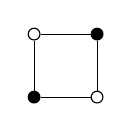
\begin{tikzpicture}[
    baseline=-3ex,
    scale=0.8,
    every node/.style={circle, draw, inner sep=1.5pt, font=\scriptsize}
]

\node[fill=black] (0) at (0,0) {};
\node[fill=white] (1) at (0,-1) {};
\node[fill=black] (2) at (-1,-1) {};
\node[fill=white] (3) at (-1,0) {};

\draw (0) -- (1) -- (2) -- (3) -- (0);

\end{tikzpicture} and 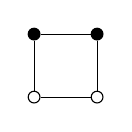
\begin{tikzpicture}[
    baseline=-3ex,
    scale=0.8,
    every node/.style={circle, draw, inner sep=1.5pt, font=\scriptsize}
]

\node[fill=black] (0) at (0,0) {};
\node[fill=white] (1) at (0,-1) {};
\node[fill=white] (2) at (-1,-1) {};
\node[fill=black] (3) at (-1,0) {};

\draw (0) -- (1) -- (2) -- (3) -- (0);

\end{tikzpicture} up to rotations and color choice.

\end{proof}
%%%%%%%%%%%%%%%%%%%%%%%%%%%%%%%%%%%%%%%%%%%%%%%%%%%%%%%%%%%% 15(b) %%%%%%%%%%%%%%%%%%%%%%%%%%%%%%%%%%%%%%%%%%%%%%%%%%%
\newpage
\setcounter{thm}{14}
\renewcommand{\thethm}{\arabic{thm}(b)}
% Sets the counter to 8(a)
\begin{prob}
Consider the cube under rotation where the faces have been colored black and
white. Find the generating function for the number of orbits by the number
of white and number of black faces in two ways: by using Theorem 6.4.2 and
by making a direct count.
\end{prob}

\begin{proof}
Earlier we found the cycle index polynomial for this action on faces of a cube to be

\[
Z(S_{4};a_1,a_2,a_3,a_4,a_5,a_6)
= \frac{1}{24}\Big(
  a_1^6
  + 6 a_1^2 a_4
  + 3 a_1^2 a_2^2
  + 8 a_3^2
  + 6 a_2^3
\Big).
\]
 So we just use $y=\{y_{1},y_{2}\}$ to plug in $a_{i}=(y_{1}^{i}+y_{2}^{i}),\forall i\in [6]$ to obtain the following after simplification
\begin{align*}
&Z(S_4;y_1+y_2,y_1^2+y_2^2,y_1^3+y_2^3,y_1^4+y_2^4,y_1^5+y_2^5,y_1^6+y_2^6)\\
&=\frac{1}{24}\Big(
(y_1+y_2)^6
+6(y_1+y_2)^2(y_1^4+y_2^4)
+3(y_1+y_2)^2(y_1^2+y_2^2)^2\\
&\qquad\qquad
+8(y_1^3+y_2^3)^2
+6(y_1^2+y_2^2)^3
\Big)\\
&=
y_1^6+y_1^5y_2+2y_1^4y_2^2
+3y_1^3y_2^3
+2y_1^2y_2^4+y_1y_2^5+y_2^6.
\end{align*}
the generating function we want where $[y_{1}^{i}y_{2}^{j}]$ counts the number of orbits with $i$ faces color $1$ and $j$ faces color $2$.

To begin counting directly, clearly there is only one way to color all faces black or white, one way to color all faces but one black or white up to rotations. Then for coloring two faces with one color up to rotation, either both faces of the same color are adjacent or opposite, so two ways. Lastly for three faces, we can color three faces in a row, or three faces adjacent forming a corner. These arent distinct orbits for each color, since two monochromatic rows are formed, or two monochromatic corners are formed. Once again, we obtain:
$$y_1^6+y_1^5y_2+2y_1^4y_2^2
+3y_1^3y_2^3
+2y_1^2y_2^4+y_1y_2^5+y_2^6.$$
\end{proof}
%%%%%%%%%%%%%%%%%%%%%%%%%%%%%%%%%%%%%%%%%%%%%%%%%%%%%%%%%%%% 30(a) %%%%%%%%%%%%%%%%%%%%%%%%%%%%%%%%%%%%%%%%%%%%%%%%%%%
\newpage
\setcounter{thm}{30}
\renewcommand{\thethm}{\arabic{thm}(a)}
\begin{prob}
Prove that $e^{\frac{2k\pi i}{n}}$ is a primitive nth root of unity if and only if $\gcd(k,n) = 1$.
\end{prob}
\begin{proof}
$(\implies)$ If $e^{\frac{2k\pi i}{n}}$ is a primitive nth root of unity, then $(e^{\frac{2k\pi i}{n}})^{m}\neq 1,\;\text{ for all } 0<m<n$. Now suppose $\gcd(k,n)=d>1.$ Then, $\ZZ^{+}\ni\frac{n}{d}<n$ and $(e^{\frac{2k\pi i}{n}})^{\frac{n}{d}}=(e^{2k\pi i})^{\frac{1}{d}}=(e^{2\pi i})^{\frac{k}{d}}=1$ since $\frac{k}{d}\in \ZZ$, a contradiction. So $\gcd(k,n) = 1$.

$(\impliedby)$ If $\gcd(k,n) = 1$, then $|k|_{\ZZ_{n}}=n$. Clearly $e^{\frac{2\pi i}{n}}$ is a primitive $nth$ root of unity, so $\langle e^{\frac{2\pi i}{n}}\rangle\cong \ZZ_{n}\implies 1\longleftrightarrow e^{\frac{2\pi i}{n}}$ is an isomorphism and then $|k|_{\ZZ_{n}}=|(e^{\frac{2\pi i}{n}})^{k}|=n$ as a result and so by definition $e^{\frac{2\pi i}{n}}$ must be a a primitive nth root of unity.

\end{proof}

%%%%%%%%%%%%%%%%%%%%%%%%%%%%%%%%%%%%%%%%%%%%%%%%%%%%%%%%%%%% 30(a) %%%%%%%%%%%%%%%%%%%%%%%%%%%%%%%%%%%%%%%%%%%%%%%%%%%

\newpage
\setcounter{thm}{30}
\renewcommand{\thethm}{\arabic{thm}(b)}
\begin{prob}
Prove that the CSP is exhibited by the triple
$$\left(\binom{[n]}{k},
\langle (1\,2\,\cdots\,n)\rangle,
\begin{bmatrix}
n\\
k
\end{bmatrix}_q \right).$$
\end{prob}

\begin{proof}
Let $X=\binom{[n]}{k}, c=(1\,2\,\cdots\,n), \omega=e^{2\pi i/n}$. We show that for each $d\geq 0$,
$$
\left|\{S\in X:c^d(S)=S\}\right|
=
\begin{bmatrix}n\\ k\end{bmatrix}_{q}\Big|_{q=\omega^d}.
$$
Fix some $d\geq 0$. Earlier we proved that $c^d$ decomposes into $m=\gcd(n,d)$ cycles, each of length $\ell=\frac{n}{m}$.

Suppose that then some cycle $(b_{1}\cdots b_{\ell})$ in the decomposition of $c^{d}$ is only partially contained in $S$ and without loss of generality there exists a first consecutive pair $(b_{i},b_{j})$ such that $b_{i}\in S,b_{j}\notin S$. So then $b_{i}$ is sent outside of $S$ which then can't be fixed by $c^{d}$. On the other hand if it is a union of cycles in $c^{d}$ then of course everything is fixed, because it only travels within a block of $S$.

So any subset \(S\in \binom{[n]}{k}\) is fixed by \(c^d\) if and only if it is some union of cycles (orbits) in the decomposition of $c^d$. That is if some subset of the cycles in $c^{d}$ viewed as a collection of blocks partitions $S$. Therefore, if \(\ell\nmid k\), then no such fixed subset exists, because it couldn't be partitioned into blocks of size $\ell$, the length of cycles in the decomposition of $c^{d}$. If \(\ell\mid k\), then \(k=\ell r\) for some $r\in \ZZ^{+}$ and all $c^{d}$-fixable \(S\) are obtained by distinctly choosing \(r=\frac{k}{\ell}\) of the \(m\) cycles. Therefore,
\[
\left|\{S\in X:c^d(S)=S\}\right|
=
\begin{cases}
\binom{m}{\frac{k}{\ell}}, & \ell\mid k,\\
0, & \ell\nmid k.
\end{cases}
\]

Now \(\omega^d\) has order $\ell=\frac{n}{\gcd(n,d)}.$ So \((\omega^d)^j=1\) if and only if \(\ell\mid j\). Observe.
\begin{align*}
\begin{bmatrix}n\\ k\end{bmatrix}_{q}\Big|_{q=\omega^d}
&=
\frac{(1-(\omega^d)^n)(1-(\omega^d)^{n-1})\cdots(1-(\omega^d)^{n-k+1})}
{(1-\omega^d)(1-(\omega^d)^2)\cdots(1-(\omega^d)^k)}.
\end{align*}

So if \(\ell\nmid k\), then among
\(
n,n-1,\dots,n-k+1
\)
there are
\(
\left\lceil \frac{k}{\ell}\right\rceil
=
\left\lfloor \frac{k}{\ell}\right\rfloor+1
\)
multiples of \(\ell\), since \(n\) itself is divisible by \(\ell\). But among
\(
1,2,\dots,k
\)
there are only
\(
\left\lfloor \frac{k}{\ell}\right\rfloor
\)
multiples of \(\ell\) since it is not. So the numerator contains exactly one more vanishing factor than the denominator and $\begin{bmatrix}n\\ k\end{bmatrix}_{q}\Big|_{q=\omega^d}=0.$

If \(\ell\mid k\), we have that $n=\ell a, k=\ell b$ for some $a,b\in \ZZ^{+}$ and then
\begin{align*}
\begin{bmatrix}n\\ k\end{bmatrix}_{q}\Big|_{q=\omega^d}
&=
\frac{(1-q^{\ell a})(1-q^{\ell(a-1)})\cdots(1-q^{\ell(a-b+1)})}
{(1-q^\ell)(1-q^{2\ell})\cdots(1-q^{b\ell})}\Bigg|_{q=\omega^d}=
\frac{a(a-1)\cdots(a-b+1)}
{1\cdot2\cdots b} = \binom{a}{b}\\
&= \binom{n/\ell=gcd(n,d)=m}{k/\ell}.
\end{align*}
Therefore
$
\left|\{S\in X:c^d(S)=S\}\right|
=
\begin{bmatrix}n\\ k\end{bmatrix}_{q}\Big|_{q=\omega^d}
$ for all \(d\geq 0\) and
$
(
\binom{[n]}{k},
\langle(1\,2\,\cdots\,n)\rangle,
\begin{bmatrix}n\\ k\end{bmatrix}_{q}
)
$ exhibits the cyclic sieving phenomenon.

\end{proof}

\end{document}